% !Mode:: "TeX:UTF-8"
% 博士范例的整本对拍件：照《研究生学位论文书写范例（理工类）》（d-stem.docx）的
% 段落序列排，章号照它 1 / 4 / 6，没有符号表、缩略语、附录、索引（范例没有）。
% 靶子是按指南把范例改齐后让 Word 排的 PDF（修正脚本 fix-doctor.py 与靶子的来路见
% tests/pages-doctor.tsv 头注释），逐行对拍 make pages-doctor。内容以范例为准，别改成示例。
\documentclass[stage=final,degree-level=doctor,campus=harbin,fontset=windows]{hithesis}
\graphicspath{{figures/}}

\hitsetup{
  info={
    secrecy={公开},
    school-code={×××},
    classified-index={××××},
    udc={××××},
    title={局部多孔质气体静压轴承关键技术的研究}[RESEARCH ON KEY TECHNOLOGIES OF PARTIAL POROUS EXTERNALLY PRESSURIZED GAS BEARING],
    author={□□□}[□□□],
    supervisor={□□□教授}[Prof. □□□],
    speciality={机械制造及其自动化}[Mechanical Manufacturing and Automation],
    affiliation={机电工程学院}[School of Mechatronics Engineering],
    date-zh={2020-06},date-en={2020-06},
    keywords={多孔质石墨, ……, 稳定性}[{porous graphite, …, Stability}],
  },
}

\hitsetup{ gb7714 = { show-note = true } }

% 第 6 章那张表后面范例留的空段数（章节文件两份共用，这个数各是各的）
\newcommand\sampleEntersAfterTable{13}
% 图 1-1 换写法的那张示范图：博士范例带题注、仍编 1-1
\newcommand\sampleAltFigureCaption{%
  \addtocounter{figure}{-1}%
  \caption{气体润滑轴承的分类}[Classification of the gas-lubricated bearing]}
\begin{document}
% 范例的参考文献表是手打的六条，正文里只引了一条；六条都排
\nocite{*}
% 范例封面的英文题目是小二（iota 的对拍件同样强制 title-en-xiaoer: true）
\cover[title-en-xiaoer]
\titlepage
% !Mode:: "TeX:UTF-8"
\begin{abstract}
气体静压轴承由于具有运动精度高、摩擦损耗小、发热变形小、寿命长、无污染等特点，在航空航天工业、半导体工业、纺织工业和测量仪器中得到广泛应用。本文在分析国内外气体静压轴承的基础上，以改善气体静压轴承的静态特性和稳定性为目的，通过理论分析、仿真计算和实验研究对局部多孔质气体静压止推轴承进行了研究，同时分析轴承的结构参数和工作参数对局部多孔质气体静压止推轴承工作特性的影响，为局部多孔质气体静压轴承的设计和工程应用奠定理论基础。

建立基于分形几何理论的多孔质石墨渗透率与分形维数之间关系的数学模型，该模型可预测多孔质石墨的渗透率，并可直观描述孔隙的大小对渗透率的影响。

本文在理论分析的基础上，建立局部多孔质气体静压止推轴承静态特性的数学模型，在此基础上，通过工程方法和有限元方法对所建立的模型进行求解。在采用有限元方法时，首先通过加权余量法，将二阶偏微分方程降为一阶，从而，降低了对插值函数连续度的要求，同时，方便采用有限元方法进行求解。

……
\end{abstract}

\begin{abstract}[lang=en]
Externally pressurized gas bearing has been widely used in the field of aviation, semiconductor, weave, and measurement apparatus because of its advantage of high accuracy, little friction, low heat distortion, long life-span, and no pollution. In this thesis, based on the domestic and overseas researching development about externally pressurized gas bearing, the author investigated the partial porous externally pressurized gas thrust bearing by theoretical analysis, computer simulation, and experiments to improve its static charaterictics and stability. The effects of structure and operating parameters on partial porous externally pressurized gas bearing has been studied. Therefore, a theoretical foundation for the designing and application for the partial porous externally pressurized gas bearing has been presented.

Based on the fractal theory, a model was established to demonstrate the relationship between the porous graphite permeability and the fractal dimension. It can predict the permeability of porous graphite and show the effects of the pore size on the permeability.

In this thesis, the author established a model about the static characteristics of partial porous externally pressurized gas thrust bearing, and it was analyzed by engineering solution and Finite Element Method (FEM). While using FEM, the second-order partial differential equation was reduced to one-order by adopting Galerkin weighted residual method, for decreasing the continuity degree requirement of the interpolation function and facilitating to the calculation.

…
\end{abstract}

\tableofcontents
% !Mode:: "TeX:UTF-8"
% 正文三章，照范例的段落序列；章号 1 / 4 / 6、节号跳着来也照它

\chapter{绪论}[Introduction]

\section{课题背景及研究的目的和意义}[Background, objective and significance of the subject]

发展国防工业、微电子工业等尖端技术需要精密和超精密的仪器设备，精密仪器设备要求高速、……

……

\section{气体润滑轴承及其相关理论的发展概况}[Developmental of gas-lubricated bearing and correlated theories]

气体轴承是利用气膜支撑负荷或减少摩擦的机械构件。……

……

\subsection{气体润滑轴承的发展}[Developmental of gas-lubricated bearing]

1828年，R.R.Willis\cite{zhao1998}发表了一篇关于小孔节流平板中压力分布的文章，这是有记载的研究气体润滑的最早文献。……

根据间隙内气膜压力的产生原理，气体轴承可以分为四种基本形式：

（1）气体静压轴承\quad 加压气体经过节流器进入间隙，在间隙内产生压力气膜使物体浮起的气体轴承，……

\subsection{气体润滑轴承的分类}[Classification of gas-lubricated bearing]

根据间隙内气膜压力的产生原理，气体轴承可以分为四种基本形式，其结构如图\ref{fig:1-1}所示。

（1）气体静压轴承\quad 加压气体经过节流器进入间隙，在间隙内产生压力气膜使物体浮起的气体轴承，结构如图\ref{fig:1-1} (a)所示。……

……

\begin{figure}[!ht]
  \centering
  \begin{minipage}{\textwidth}
    \centering
    \subfigure[]{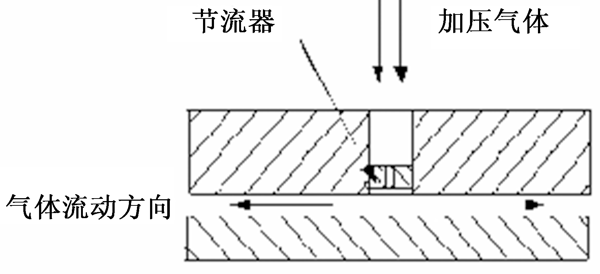
\includegraphics[width=6.92cm]{aerostatic}}
    \hspace{1cm}
    \subfigure[]{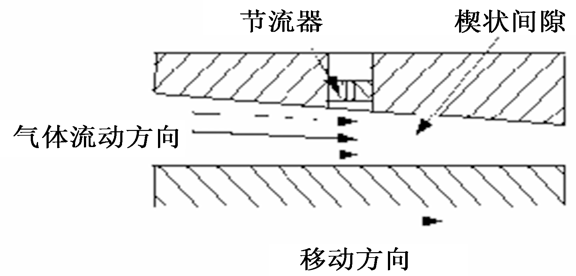
\includegraphics[width=6.65cm]{aerodynamic}}
  \end{minipage}
  \begin{minipage}{\textwidth}
    \centering
    \subfigure[]{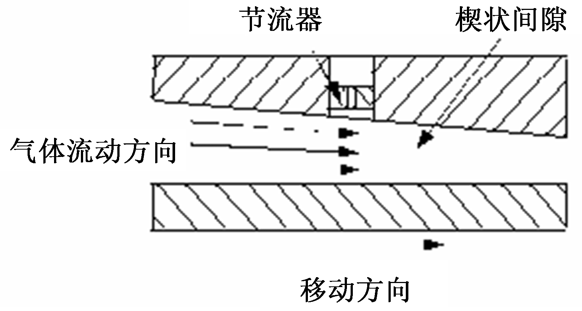
\includegraphics[width=6.72cm]{hybrid}}
    \hspace{1cm}
    \subfigure[]{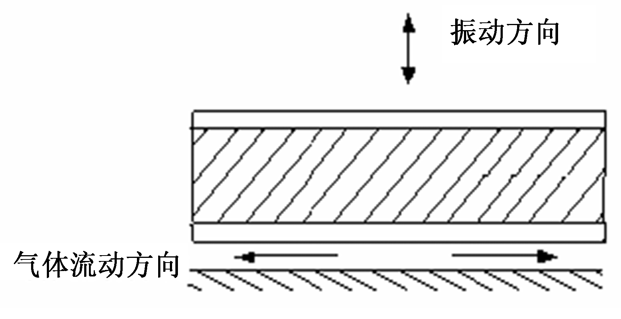
\includegraphics[width=7.71cm]{squeeze-film}}
  \end{minipage}
  \caption{气体润滑轴承的分类}[Classification of the gas-lubricated bearing]
  \label{fig:1-1}

  {\wuhao (a) 气体静压轴承; (b) 气体动压轴承; (c) 气体动静压轴承; (d) 气体压膜轴承\par}
\end{figure}

（也可以按照下图范例书写）

\begin{figure}[!ht]
  \centering
  \subfigure[气体静压轴承]{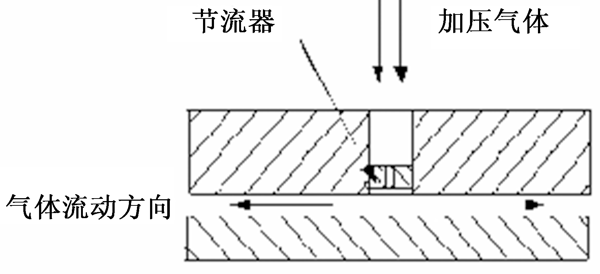
\includegraphics[width=6.87cm]{aerostatic}}
  \hspace{1cm}
  \subfigure[气体动压轴承]{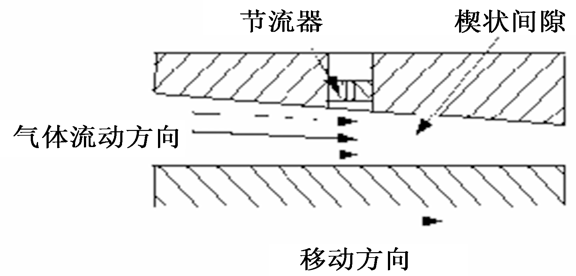
\includegraphics[width=6.03cm]{aerodynamic}}
  \caption{气体润滑轴承的分类}[Classification of the gas-lubricated bearing]
  \label{fig:1-2}
\end{figure}

\clearpage

\begin{figure}[!ht]
  \centering
  \addtocounter{figure}{-1}
  \addtocounter{subfigure}{2}
  \subfigure[气体动静压轴承]{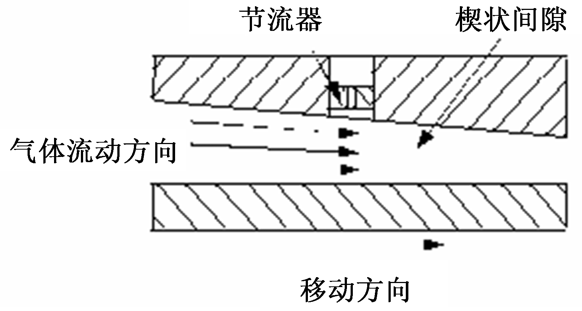
\includegraphics[width=6.70cm]{hybrid}}
  \hspace{1cm}
  \subfigure[气体压膜轴承]{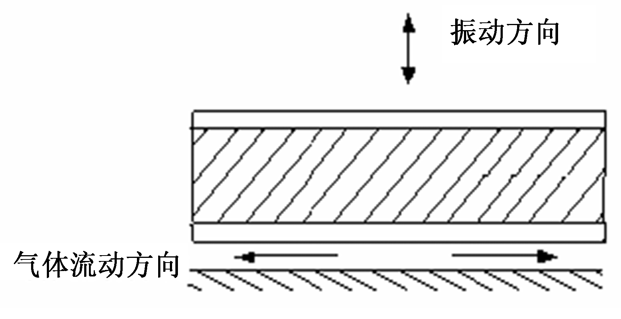
\includegraphics[width=7.17cm]{squeeze-film}}
  \caption*{图\thefigure（续图）}
\end{figure}

\setcounter{subsection}{4}
\subsection{多孔质气体静压轴承的研究}[Research on porous externally pressurized gas bearing]

由于气体的压力低和可压缩性，……。

\subsubsection{多孔质静压轴承的分类}[Classification of porous thrust bearing]

轴承工作面的整体或……。

\subsubsection{多孔质材料特性的研究}[Research on characteristics of porous materials]

材料的主要特点是具有一定的……。

（1）孔隙特性\quad 多孔质材料是由……。

……

\setcounter{section}{3}
\section{本文的主要研究内容}[Main research content of this subject]

本课题的研究内容主要是针对局部多孔质止推轴承的多孔质材料的渗透率、静压轴承的静态特性、稳定性及其影响因素进行展开，……。

\setcounter{chapter}{3}
\chapter{基于FLUENT软件的轴承静态特性研究}[Research on static characteristics of bearing based on FLUENT software]

\section{引言}[Introduction]

利用现成的商用软件来研究流场，可以免去对N-S方程求解程序的……

\setcounter{section}{2}
\setcounter{subsection}{2}
\subsection{边界条件的设定}[Initialization of boundary conditions]

本文采用……，则每一个方向上的……由公式\eqref{eq:4-1}、\eqref{eq:4-2}求得：
\begin{equation}\label{eq:4-1}
  \alpha = \frac{D_{\mathrm{p}}^2}{150}\frac{\psi^3}{(1-\psi)^2}
\end{equation}
\begin{equation}\label{eq:4-2}
  C_2 = \frac{3.5}{D_{\mathrm{p}}}\frac{(1-\psi)}{\psi^3}
\end{equation}
\begin{eqdenote}
  \item $D_{\mathrm{p}}$ & 多孔质材料的平均粒子直径（m）；
  \item $\psi$ & 孔隙度（孔隙体积占总体积的百分比）；
  \item $C_2$ & 特征渗透性或固有渗透性（m$^2$）。
\end{eqdenote}

……

\setcounter{section}{3}
\section{本章小结}[Brief summary]

……

\setcounter{chapter}{5}
\chapter{局部多孔质静压轴承的试验研究}[Experiment on partial porous thrust bearing]

\section{引言}[Introduction]

在前面几章中，分别对局部多孔质材料的渗透率……

\section{多孔质石墨渗透率测试试验}[Experiments on permeability of porous graphite]

……

1号试样的试验数据见表\ref{tab:6-1}。

\begin{table}[!ht]
  \centering
  \caption{1号试样渗透率测试数据(温度：$T$=16 ℃\quad 高度：$H$=5.31 mm)}[Data of measured permeability of sample 1 (Temperature: $T$=16 ℃\quad Height: $H$=5.31 mm)]
  \label{tab:6-1}
  \begin{tblr}{colspec={X[c]X[c]X[c]X[c]X[c]X[c]}, width=\textwidth}
    \toprule
    {供气压力\\ $P_{\mathrm{s}}$ (MPa)} & {流量测量\\ $M'$ (m$^3$/h)} & {流量修正值 $M$ (m$^3$/s)\\ $\times$10$^{-4}$} & {压力差\\ $\Delta P$ (Pa)} & lg$\Delta P$ & lg $M$ \\
    \midrule
    0.15 & 0.009 & 0.023 12 & 46 900 & 4.671 17 & -5.636 01 \\
    0.2 & 0.021 & 0.045 84 & 96 900 & 4.986 32 & -5.338 76 \\
    0.25 & 0.039 & 0.074 13 & 146 900 & 5.167 02 & -5.130 01 \\
    0.3 & 0.097 & 0.167 47 & 196 900 & 5.294 24 & -4.776 06 \\
    0.35 & 0.136 & 0.217 53 & 246 900 & 5.392 52 & -4.662 48 \\
    0.4 & 0.171 & 0.254 85 & 296 900 & 5.472 61 & -4.593 72 \\
    0.45 & 0.202 & 0.284 67 & 346 900 & 5.540 20 & — \\
    \bottomrule
  \end{tblr}
\end{table}

% 范例在这行前留了十三个空段，Word 排到下一页顶上还剩四个空行；照它空四行
\clearpage
\hitenter*[4]

……如果表格超过一页时，可采用续表的形式移入下一页：

\addtocounter{table}{-1}
\begin{longtblr}[
  caption={试样渗透率测试数据},
  caption-en={Data of measured permeability of sample 1},
  label={tab:6-1b}]{colspec={X[c]X[c]X[c]X[c]X[c]X[c]}, width=\textwidth}
  \toprule
  {供气压力\\ $P_{\mathrm{s}}$ (MPa)} & {流量测量\\ $M'$ (m$^3$/h)} & {流量修正值 $M$ (m$^3$/s)\\ $\times$10$^{-4}$} & {压力差\\ $\Delta P$ (Pa)} & lg$\Delta P$ & lg $M$ \\
  \midrule
  0.15 & 0.009 & 0.023 12 & 46 900 & 4.671 17 & -5.636 01 \\
  0.2 & 0.021 & 0.045 84 & 96 900 & 4.986 32 & -5.338 76 \\
  0.25 & 0.039 & 0.074 13 & 146 900 & 5.167 02 & -5.130 01 \\
  0.15 & 0.009 & 0.023 12 & 46 900 & 4.671 17 & -5.636 01 \\
  0.2 & 0.021 & 0.045 84 & 96 900 & 4.986 32 & -5.338 76 \\
  0.25 & 0.039 & 0.074 13 & 146 900 & 5.167 02 & -5.130 01 \\
  0.15 & 0.009 & 0.023 12 & 46 900 & 4.671 17 & -5.636 01 \\
  0.2 & 0.021 & 0.045 84 & 96 900 & 4.986 32 & -5.338 76 \\
  0.25 & 0.039 & 0.074 13 & 146 900 & 5.167 02 & -5.130 01 \\
  0.15 & 0.009 & 0.023 12 & 46 900 & 4.671 17 & -5.636 01 \\
  0.2 & 0.021 & 0.045 84 & 96 900 & 4.986 32 & -5.338 76 \\
  0.25 & 0.039 & 0.074 13 & 146 900 & 5.167 02 & -5.130 01 \\
  0.15 & 0.009 & 0.023 12 & 46 900 & 4.671 17 & -5.636 01 \\
  0.2 & 0.021 & 0.045 84 & 96 900 & 4.986 32 & -5.338 76 \\
  0.25 & 0.039 & 0.074 13 & 146 900 & 5.167 02 & -5.130 01 \\
  0.15 & 0.009 & 0.023 12 & 46 900 & 4.671 17 & -5.636 01 \\
  0.2 & 0.021 & 0.045 84 & 96 900 & 4.986 32 & -5.338 76 \\
  0.25 & 0.039 & 0.074 13 & 146 900 & 5.167 02 & -5.130 01 \\
  $\vdots$ & & & & & \\
  0.3 & 0.097 & 0.167 47 & 196 900 & 5.294 24 & -4.776 06 \\
  0.35 & 0.136 & 0.217 53 & 246 900 & 5.392 52 & -4.662 48 \\
  0.4 & 0.171 & 0.254 85 & 296 900 & 5.472 61 & -4.593 72 \\
  0.45 & 0.202 & 0.284 67 & 346 900 & 5.540 20 & — \\
  \bottomrule
\end{longtblr}

\setcounter{section}{4}
\section{本章小结}[Brief summary]

……

% !Mode:: "TeX:UTF-8"
\begin{conclusions}
本文对局部多孔质气体静压止推轴承的静态特性和稳定性进行了理论研究，对于局部多孔质气体静压径向轴承、圆锥轴承和球轴承仅需对止推轴承压力分布的数学模型进行适当的坐标变换即可对其特性进行求解。同时，本文对局部多孔质气体静压止推轴承进行了实验研究并与整体多孔质和小孔节流止推轴承的静态特性和稳定性进行了实验对比。

本论文的主要创造性工作归纳如下：

1. 建立了基于分形几何理论的多孔质石墨渗透率与分形维数之间关系的数学模型，该模型可预测多孔质石墨的渗透率，并可直观描述各种孔隙的大小对渗透率的影响。通过实验验证了该模型的正确性。

2. 分别建立了基于气体连续性方程、Navier-Stokes 方程、Darcy 定律以及气体状态方程的局部多孔质气体静压轴承的承载能力、静态刚度和质量流量的数学模型，利用有限元法进行求解，给出了局部多孔质气体静压轴承的承载能力、静态刚度和质量流量特性曲线。

……

今后还应在以下几个方面继续深入研究：

1. 本文仅是采用了局部多孔质圆柱塞这种节流方式，在以后的研究中，可以通过改变局部多孔质材料的形状来改变节流方式，从而通过性能对比，获得最优的节流效果。

……
\end{conclusions}

\bibliography{refs}
% !Mode:: "TeX:UTF-8"
% 范例的成果页：三组，条目从 pub.bib 出
\begin{achievements}[pub]
  \begin{pubgroup}{发表的学术论文}
    \item{pub:1}
    \item{pub:2}
    \item{pub:3}
    \item{pub:4}
    \item{pub:5}
    \item{pub:6}
  \end{pubgroup}
  \begin{pubgroup}{申请及已获得的专利（无专利时此项不必列出）}
    \item{pub:patent}
  \end{pubgroup}
  \begin{pubgroup}{参与的科研项目及获奖情况}
    \item{pub:proj}
    \item{pub:award}
  \end{pubgroup}
\end{achievements}

\defense
\declarations
% !Mode:: "TeX:UTF-8"
\begin{acknowledgements}
衷心感谢导师×××教授对本人的精心指导。他的言传身教将使我终身受益。

感谢×××教授，以及实验室全体老师和同窗们的热情帮助和支持！

本课题承蒙××××基金资助，特此致谢。

……
\end{acknowledgements}

% !Mode:: "TeX:UTF-8"
\begin{resume}
××××年××月××日出生于××××。

××××年××月考入××大学××院（系）××专业，××××年××月本科毕业并获得××学学士学位。

××××年××月——××××年××月，在××大学××院（系）××学科学习并获得××学硕士学位。

××××年××月——××××年××月，在××大学××院（系）××学科攻读博士学位。

获奖情况：如获三好学生、优秀团干部、×奖学金等（不含科研学术获奖）。

工作经历：

\textbf{（个人简历一般应包含从本科起的教育经历和工作经历）}
\end{resume}

\end{document}
